% Format teze zasnovan je na paketu memoir
% http://tug.ctan.org/macros/latex/contrib/memoir/memman.pdf ili
% http://texdoc.net/texmf-dist/doc/latex/memoir/memman.pdf
% 
% Prilikom zadavanja klase memoir, navedenim opcijama se podešava 
% veličina slova (12pt) i jednostrano štampanje (oneside).
% Ove parametre možete menjati samo ako pravite nezvanične verzije
% mastera za privatnu upotrebu (na primer, u b5 varijanti ima smisla 
% smanjiti 
\documentclass[12pt,oneside]{memoir} 

% Paket koji definiše sve specifičnosti master rada Matematičkog fakulteta
\usepackage[latinica]{matfmaster} 
\usepackage{elm-highlighting}

\usepackage{listings,xcolor}
    \usepackage[T1]{fontenc}
    \usepackage{xcolor}
    \usepackage[scaled=0.9]{DejaVuSansMono}
\definecolor{commentgreen}{RGB}{2,112,10}
\definecolor{eminence}{RGB}{108,48,130}
\definecolor{weborange}{RGB}{255,165,0}
\definecolor{frenchplum}{RGB}{129,20,83}

\lstdefinelanguage{elixir}{
    morekeywords={case,catch,def,do,else,false,%
        use,alias,receive,timeout,defmacro,defp,%
        for,if,import,defmodule,defprotocol,%
        nil,defmacrop,defoverridable,defimpl,%
        super,fn,raise,true,try,end,with,%
        unless},
    otherkeywords={<-,->, |>, \%\{, \}, \{, \, (, )},
    sensitive=true,
    morecomment=[l]{\#},
    morecomment=[n]{/*}{*/},
    morecomment=[s][\color{purple}]{:}{\ },
    morestring=[s][\color{orange}]"",
    commentstyle=\color{commentgreen},
    keywordstyle=\color{eminence},
    stringstyle=\color{red},
	basicstyle=\ttfamily,
	breaklines,
	showstringspaces=false,
	frame=tb
}


%

%

%
% Opcija [biblatex]:
%   ako želite da koristite reference na više jezika i umesto paketa
%   bibtex da koristite BibLaTeX/Biber, dodajte opciju "biblatex" tj.
%   prethodni paket uključite pomoću: \usepackage[biblatex]{matfmaster}
%
% Opcija [b5paper]:
%   ako želite da napravite verziju teze u manjem (b5) formatu, navedite
%   opciju "b5paper", tj. prethodni paket uključite pomoću: 
%   \usepackage[b5paper]{matfmaster}. Tada ima smisla razmisliti o promeni
%   veličine slova (izmenom opcije 12pt na 11pt u \documentclass{memoir}).
%
% Naravno, opcije je moguće kombinovati.
% Npr. \usepackage[b5paper,biblatex]{matfmaster}


% Datoteka sa literaturom u BibTex tj. BibLaTeX/Biber formatu
\bib{matfmaster-primer}

% Ime kandidata na srpskom jeziku (u odabranom pismu)
\autor{Ana Petrović}
% Naslov teze na srpskom jeziku (u odabranom pismu)
\naslov{Testiranje funkcionalnog koda}
% Godina u kojoj je teza predana komisiji
\godina{2023}
% Ime i afilijacija mentora (u odabranom pismu)
\mentor{dr Ime\textsc{Prezime}, redovan profesor\\ Univerzitet u Beogradu, Matematički fakultet}
% Ime i afilijacija prvog člana komisije (u odabranom pismu)
\komisijaA{dr Ime \textsc{Prezime}, vanredni profesor\\ University of Disneyland, Nedođija}
% Ime i afilijacija drugog člana komisije (u odabranom pismu)
\komisijaB{dr Ime \textsc{Prezime}, docent\\ Univerzitet u Beogradu, Matematički fakultet}
% Ime i afilijacija trećeg člana komisije (opciono)
% \komisijaC{}
% Ime i afilijacija četvrtog člana komisije (opciono)
% \komisijaD{}
% Datum odbrane (odkomentarisati narednu liniju i upisati datum odbrane ako je poznat)
% \datumodbrane{}

% Apstrakt na srpskom jeziku (u odabranom pismu)
\apstr{%
Apstrakt
}

% Ključne reči na srpskom jeziku (u odabranom pismu)
\kljucnereci{funkcionalno programiranje, testiranje, verifikacija softvera, programski jezik Elixir, programski jezik Elm}

\begin{document}
% ==============================================================================
% Uvodni deo teze
\frontmatter
% ==============================================================================
% Naslovna strana
\naslovna
% Strana sa podacima o mentoru i članovima komisije
\komisija
% Strana sa posvetom (u odabranom pismu)
%\posveta{Mami, tati i dedi}
% Strana sa podacima o disertaciji na srpskom jeziku
\apstrakt
% Sadržaj teze
\tableofcontents*

% ==============================================================================
% Glavni deo teze
\mainmatter
% ==============================================================================

% ------------------------------------------------------------------------------
\chapter{Uvod}
% ------------------------------------------------------------------------------

Ovde ide uvod .. ... ..... 

% ------------------------------------------------------------------------------
\chapter{Funkcionalna paradigma}
\label{chp:uvodnideo}

\par Funkcionalno programiranje je specifičan pristup programiranju, tj. programska paradigma, u kojoj se programi kreiraju pomoću izraza i matematičkih funkcija, bez izmena stanja i podataka \cite{func}. Funkcionalni programi su iz tog razloga jednostavniji za razumevanje i otporniji na greške u odnosu na imperativne. Za razliku od imperativnih jezika kod kojih je osnovna apstrakcija podrutina, ili objektno-orijentisanih objekat, u slučaju funkcionalnih programskih jezika - osnovna apstrakcija je \textit{funkcija}. Programski stil je deklarativnog tipa i umesto naredbi koriste se izrazi, tako da se izvršavanje programa svodi na evaluaciju izraza. Vrednost izraza je nezavisna od konteksta u kojem se izraz nalazi. Osnovna osobina čistih funkcionalnih jezika (eng. \textit{pure functional programming language}) jeste transparentnost referenci, što kao posledicu ima nepostojanje propratnih bočnih efekata.
\par Skoro svi funkcionalni jezici zasnovani su na \textit{lambda računu} (eng. \textit{ $\lambda$-calculus}) , čija je osnovna svrha da da definiciju izračunljivosti. Pored toga što se smatra prvim funkcionalnim jezikom, lambda račun se naziva i najmanjim programskim jezikom na svetu. Sve što se može izračunati lambda računom smatra se izračunljivim. Ekspresivnost funkcionalnih jezika ekvivalentna je ekspresivnosti Tjuringove mašine \cite{turing}. 

\section{Karakteristike funkcionalnih programa}
U nastavku su objašnjene neke od najvažnijih osobina funkcionalnih programskih jezika. 

\subsection{Čista funkcija}
Čista funkcija (eng. \textit{pure function}) ima dve osnovne karakteristike: 
\begin{itemize}
\item Uvek proizvodi isti izlaz za iste argumente, bez obzira na sve ostalo
\item Imutabilnost 
\end{itemize}
\par
Druga osobina podrazumeva da ne postoje bočni efekti, tj. čista funkcija ne vrši nikakve izmene nad argumentima, kao ni nad lokalnim ili globalnim promenljivima. Jedini rezultat čiste funkcije jeste vrednost koju ona vrati. Kao posledica ovoga, funkcionalni programi su laki za debagovanje. Čiste funkcije takođe olakšavaju paralelizaciju i konkurentnost aplikacija. Na osnovu ovako napisanih programa, kompilator lako može da paralelizuje naredbe, sačeka da evaluira rezultate kada budu potrebni, i na kraju da zapamti rezultat, s obzirom na to da se on neće promeniti sve dok ulaz ostaje isti. Kod \ref{lst:pure} prikazuje primer jedne čiste funkcije u programskom jeziku Elixir. 

\begin{lstlisting}[language=elixir, caption={Primer čiste funkcije},captionpos=b, label={lst:pure}]
defmodule Math do 
  def fibonacci(0) do 0 end
  def fibonacci(1) do 1 end
  def fibonacci(n) do fibonacci(n-1) + fibonacci(n-2) end
end

IO.puts Math.fibonacci(9)
\end{lstlisting}

\subsection{Rekurzija}
Za razliku od imperativnog programiranja, kod funkcionalno napisanih programa može se primetiti odsustvo petlji. Funkcije se definišu rekurzivno - pozivaju same sebe i time postižu ponavljanje izvršavanja. U mnogim slučajevima, umesto rekurzije se koriste funkcije višeg reda.

\subsection{Funkcije kao građani prvog reda}
U funkcionalnim programima, funkcije se smatraju građanima prvog reda (eng.\emph{ First Class Citizen}). To znači da u okviru jezika ne postoje restrikcije po pitanju njihovog kreiranja i korišćenja. Građani prvog reda su entiteti u okviru programskog jezika koji mogu biti:
\begin{itemize}
\item deo nekog izraza
\item dodeljeni nekoj promenljivoj
\item prosleđeni kao argument funkcije
\item povratne vrednosti funkcije
\end{itemize}
Mogućnost prosleđivanja funkcija kao argumenata drugih funkcija je ključna za funkcionalnu paradigmu. 

\subsection{Funkcije višeg reda}
Funkcija višeg reda je funkcija koja kao argument uzima jednu ili više funkcija i/ili ima funkciju kao svoju povratnu vrednost. U funkcionalnom programiranju postoje tri jako korisne ovakve funkcije - map, filter i reduce (fold).  Funkcija mapiranja omogućava operisanje nad jako velikim količinama podataka. Kao argumente prima funkciju i listu, i zatim primeni datu funkciju na svaki element liste i kao povratnu vrednost proizvodi novu listu. Upotrebom funkcije filter mogu se eliminisati neželjeni elementi neke liste - na osnovu prosleđene funkcije predikata i date liste, filter vraća listu sa elementima koji ispunjavaju dati kriterijum. Fold prihvata tri argumenta: funkciju spajanja, početnu vrednost i listu. Iznova primenjuje funkciju spajanja na početnu vrednost i datu listu, sve dok se rezultat ne redukuje na jednu vrednost. Primer koda \ref{lst:high} pokazuje upotrebu funkcija višeg reda u programskom jeziku Elm. Prednost korišćenja ovih funkcija je u paralelnom izvršavanju, s obzirom da funkcionalni programi nemaju stanje. Takođe, daju jako sažet i čist kod.

\begin{lstlisting}[language=elm, caption={Funkcije višeg reda},captionpos=b, label={lst:high}]
[1, 2, 3] |> List.map (\number -> number * 2) -- [2, 4, 6]
[1, 2, 3, 4, 5] |> List.filter (\number -> number <= 3) -- [1, 2, 3]
[1, 2, 3, 4, 5] |> List.foldl (\item total -> total + item) 0 -- 15
\end{lstlisting}

\subsection{Transparentnost referenci}
Jednom definisane promenljive u funkcionalnom programu ne menjaju više svoju vrednost. Programi nemaju naredbe dodele, već kada je potrebno sačuvati neku vrednost definišu se nove promenljive. Ovaj pristup eliminiše šanse za postojanje bočnih efekata jer svaka promenljiva može biti zamenjena svojom pravom vrednošću u bilo kom trenutku tokom izvršavanja programa. Stanje svake promenljive je konstantno. 

\section{Testiranje funkcionalnih programa}
\label{sec:piramid}

\par Testiranje koda je jedan od najvažnijih aspekata u procesu razvoja softvera. Softver koji ne radi onako kako je predviđen može dovesti do različitih problema, kao što su gubitak novca i vremena, ili u najgorim slučajevima - povrede ili smrti. Testiranjem se osigurava kvalitet softvera i smanjuje rizik od padova. Glavna uloga testiranja jeste provera da li sistem zadovoljava specifikacije, ali uključuje i validaciju - provera da li sistem ispunjava sve potrebe korisnika.  
\par Cilj testiranja je pronalaženje grešaka, proverom da li su ispunjeni svi funkcionalni i nefunkcionalni zahtevi \cite{test}. 

\subsection{Organizacija testova}

\par Model piramide testiranja (prikazan na slici \ref{fig:piramida}) je koncept koji pomaže u razmišljanju o tome kako testirati softver \cite{cohn}. Uloga piramide je da vizuelno predstavi logičku organizaciju standarda u testiranju. Sastoji se od 3 sloja: bazu piramide predstavljaju jedinični testovi (eng. \emph{Unit Test}). Njih bi trebalo da bude najviše - kako su najmanji, samim tim su i najbrži, a izvršavaju se u potpunoj izolaciji. Na sledećem nivou, u sredini piramide, nalaze se integracioni testovi (ili testovi servisa). Integracija podrazumeva način na koji različite komponente sistema rade zajedno. Nisu potrebne interakcije sa korisničkim interfejsom, s obzirom na to da ovi testovi pozivaju kod preko interfejsa. Vrh piramide čine testovi korisničkog interfejsa (eng. \emph{User Interface - UI}), poznati i kao E2E \footnote{E2E je skraćenica za testove sa kraja na kraj (eng. \emph{End-to-End})} testovi. Oni zahtevaju rad celokupnog sistema, pa su zbog toga prilično skupi. Potrebno je doneti odluku koje testove i koliko njih sprovesti u ovom slučaju.
\par U opštem slučaju, testiranje projekta koji se sastoji od više slojeva podrazumeva kombinaciju jediničnih, integracionih i E2E testova kako bi se osigurala ukupna funcionalnost, pouzdanost i perfomanse sistema. Pored ova tri osnovna tipa testova, postoji i testiranje opterećenja (eng.\emph{ load testing}), kojim se može proveriti da li i koliko sistem podnosi veliki broj zahteva ili korisnika. 

\begin{figure}[!ht]
  \centering
  \label{fig:piramida}
  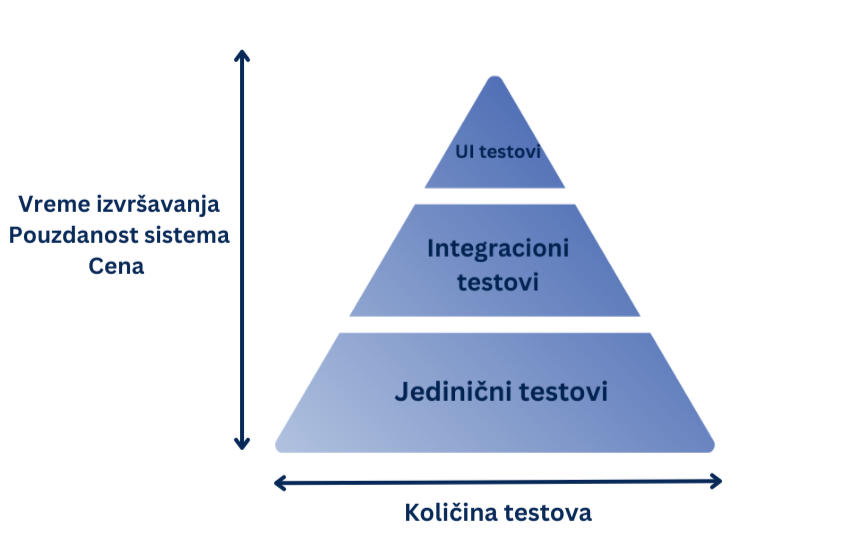
\includegraphics[width=0.8\textwidth]{piramida.png}
  \caption{Model piramide testiranja}
\end{figure}

\par 
Razvoj vođen testovima (eng. \emph{Test-Driven Develpment , TDD}) je praksa u razvoju softvera koja nalaže da se prvo napišu testovi. Ti testovi na početku ne prolaze, s obzirom na to da kod još uvek nije implementiran, a zatim se iznova pokreću tokom pisanja samog koda, sve dok ne prođu. Ova tehnika kontinualnog testiranja tokom razvoja se često preporučuje  jer se lako i veoma rano uoče greške i time sprečavaju padovi u kasnijim fazama razvoja. Ipak, u ovom radu neće biti primenjen TDD pristup. Kako je tema testiranje, fokus nije na pisanju koda aplikacije, već testova za već napisan projekat. Aplikacija koja će biti testirana služi samo kao primer na kome će biti prikazani značajni koncepti testiranja funkcionalnih programa. Kratak opis testiranog projekta biće preciznije objašnjen u poglavlju \ref{chp:msnr}. 

\par Čiste funkcije samo uzimaju argumente i proizvode neki izlaz,  ne prave nikakve izmene niti imaju neke skrivene izlaze. Koriste imutabilne vrednosti, i time olakšavaju pronalaženje nekih problema u programima. Testiranje i debagovanje ovako napisanih programa  postaje mnogo jednostavnije. Najvažnija stvar kod testiranja u funkcionalnoj paradigmi jeste pisanje čistih funkcija i njihovo testiranje u izolaciji, kako bi se obezbedila ispravnost i robustnost. 

\subsection{Testiranje čistih funkcija}
\par Najjednostavniji kod za testiranje jeste čista funkcija. Kao što je već navedeno ranije, čista funkcija uvek vraća isti rezultat za iste ulazne parametre i odlikuje je nepostojanje bočnih efekata. Dakle, ako postoji bilo kakva izmena podataka, funkcija nije čista. Pri testiranju ovakve funkcije, test može da se fokusira samo na dve stvari: ulazne podatke i na sam izlaz funkcije. 
\par Kada je u pitanju čista funkcija, jedina priprema koja je potrebna jesu podaci koji će se proslediti kao parametri. Drugi korak jeste poziv funkcije, sa prosleđenim argumentima. Faza verfikacije su samo provere nad rezultatom, i samo nad rezultatom. Testovi ne moraju da brinu o bočnim efektima i konstatno dobijaju isti odgovor od testiranog koda, ma koliko puta bili pokrenuti. Važan aspekat testiranja u funkcionalnoj paradigmi je da se ne testira samo uspešan scenario, već i granični slučajevi, kao i slučajevi greške. Kako su funkcije čiste i nemaju bočnih efekata, slučajevi se mogu lako testirati bez brige o nekim neočekivanim posledicama. 
\par Naravno, skoro nijedna aplikacija se ne može sastojati od samo čistih funkcija, i u vezi sa tim postoje dve strategije \cite{testingelixir} . Prva je izdvojiti logiku u neke čiste funkcije, a druga dizajnirati funkcije tako da koriste neku metodu ubrizgavanja zavisnosti (eng. \textit{Dependency injection}) \footnote{Ubrizgavanje zavisnosti je šablon u kom objekat ili funkcija prihvata druge objekte ili funkcije od kojih zavisi. Jedan od oblika inverzije kontrole, za cilj ima da razdvoji konstrukciju i upotrebu objekata i time smanjuje spregnutost programa.}, što omogućava izolaciju koda.

\subsubsection{Refaktorisanje ka čistim funkcijama} 
Ako je neki modul jako težak za testiranje, najlakši način da se pojednostavi jeste refaktorisati kod u čistu funkciju, ukoliko je to moguće. Deo koda koji zavisi od nekog drugog dela iz spoljašnjosti će u većini slučajeva pozivati tu spoljašnju zavisnost i onda nekako manipulisati rezultatom pre nego što vrati svoj rezultat. Što više takve manipulacije ima, to je taj deo koda bolji kandidat za premeštanje logike unutar čiste funkcije. Na slikama \ref{fig:dep1} i \ref{fig:dep2} su date vizuelne reprezentacije kako ovaj proces teče pre i posle izmeštanja koda u čistu funkciju. 
Testiranje funkcije sa prve slike može biti komplikovano. Svaki test, za svaki mogući način ponašanja bi nekako morao da garantuje da druga funkcija (ona od koje zavisi prva) vraća neki očekivani, poznati odgovor. Ideja je da se deo logike (na slici označen sa ``manipulacija podataka `` izvuče van - u novu, čistu funkciju. Tako postaje zasebna zavisnost, koja se može odvojeno lako testirati. Ovime se izbegava velika kompleksnost do koje može doći. Kada je taj deo logike dobro istestiran, može se smatrati sigurnim da se ponovo pozove u originalnoj funkciji. Zna se da će taj kod uvek vraćati isti rezultat, i može se značajno redukovati broj testova neophodnih za testiranje originalne funkcije.

\begin{figure}[!ht]
  \centering
  \label{fig:dep1}
  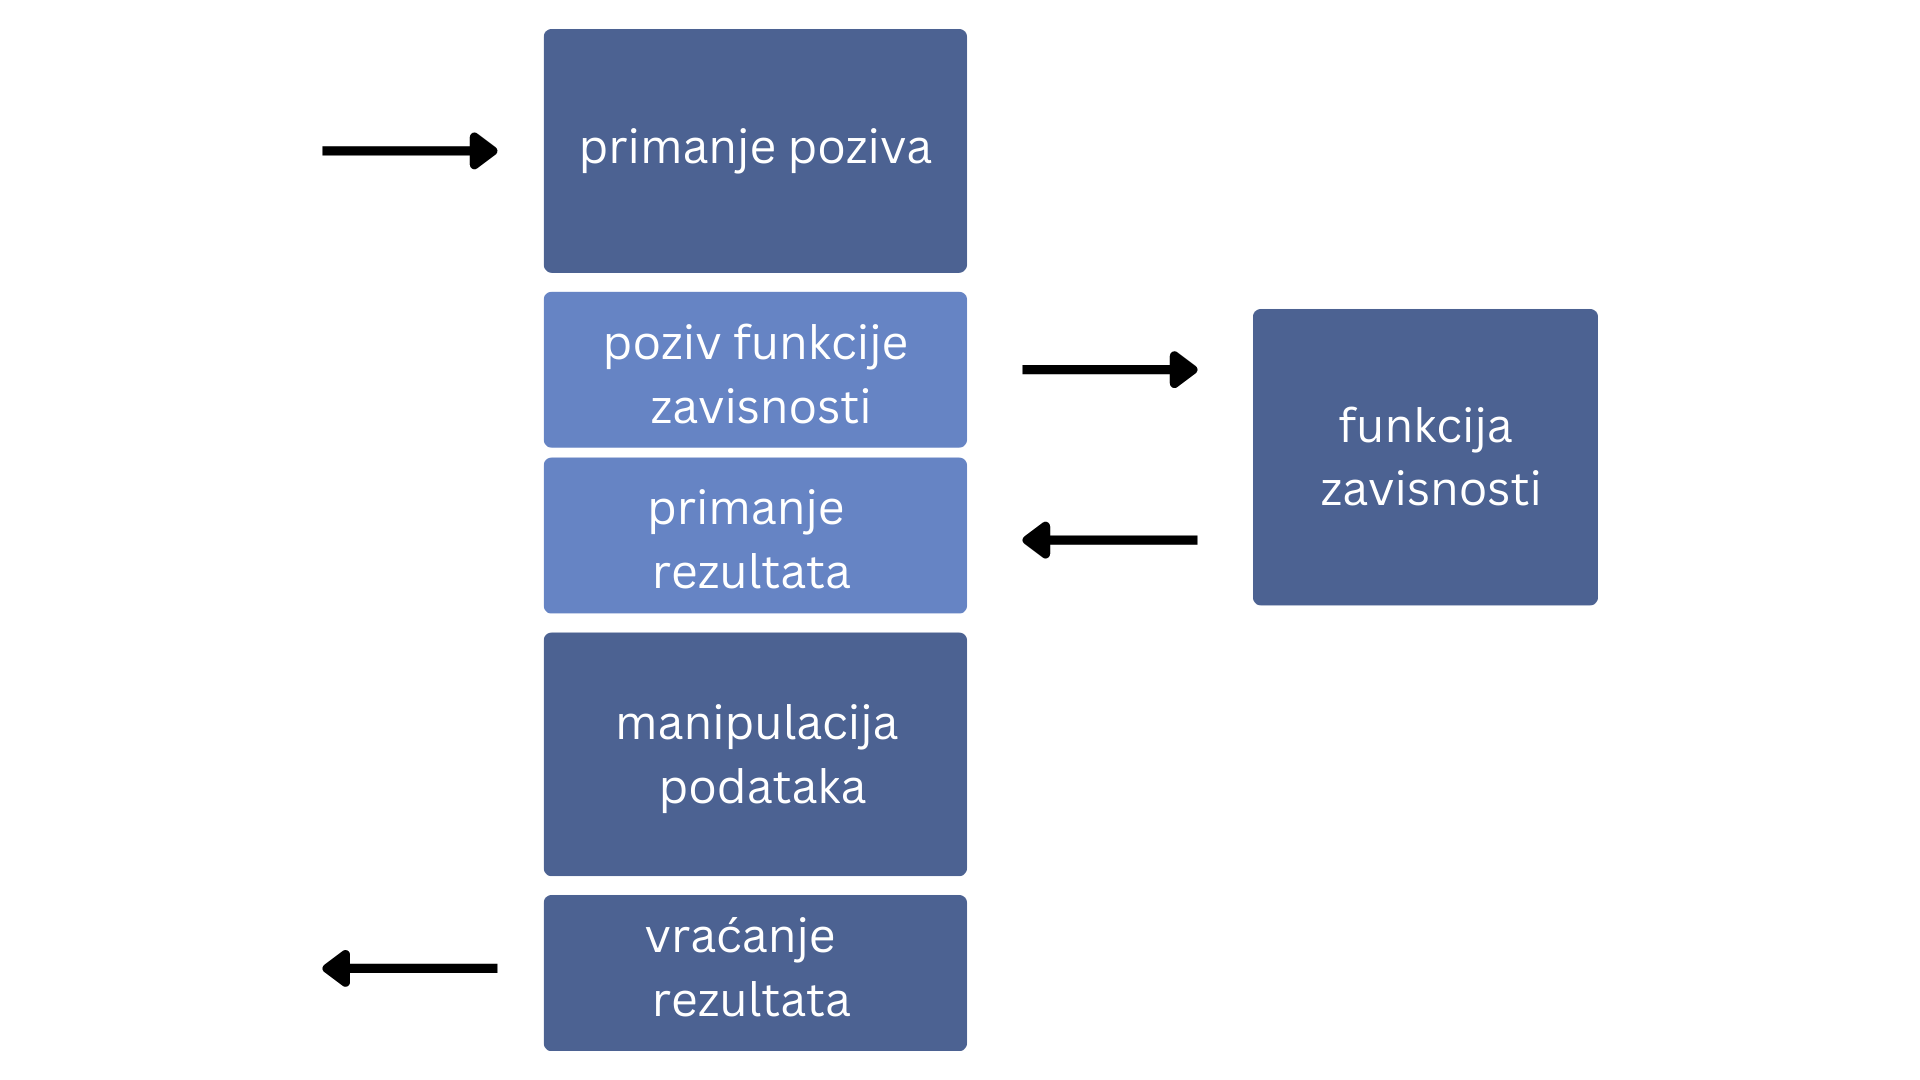
\includegraphics[width=0.6\textwidth]{dep1.png}
  \caption{Pre izmeštanja u čistu funkciju}
\end{figure}

\begin{figure}[!ht]
  \centering
  \label{fig:dep2}
  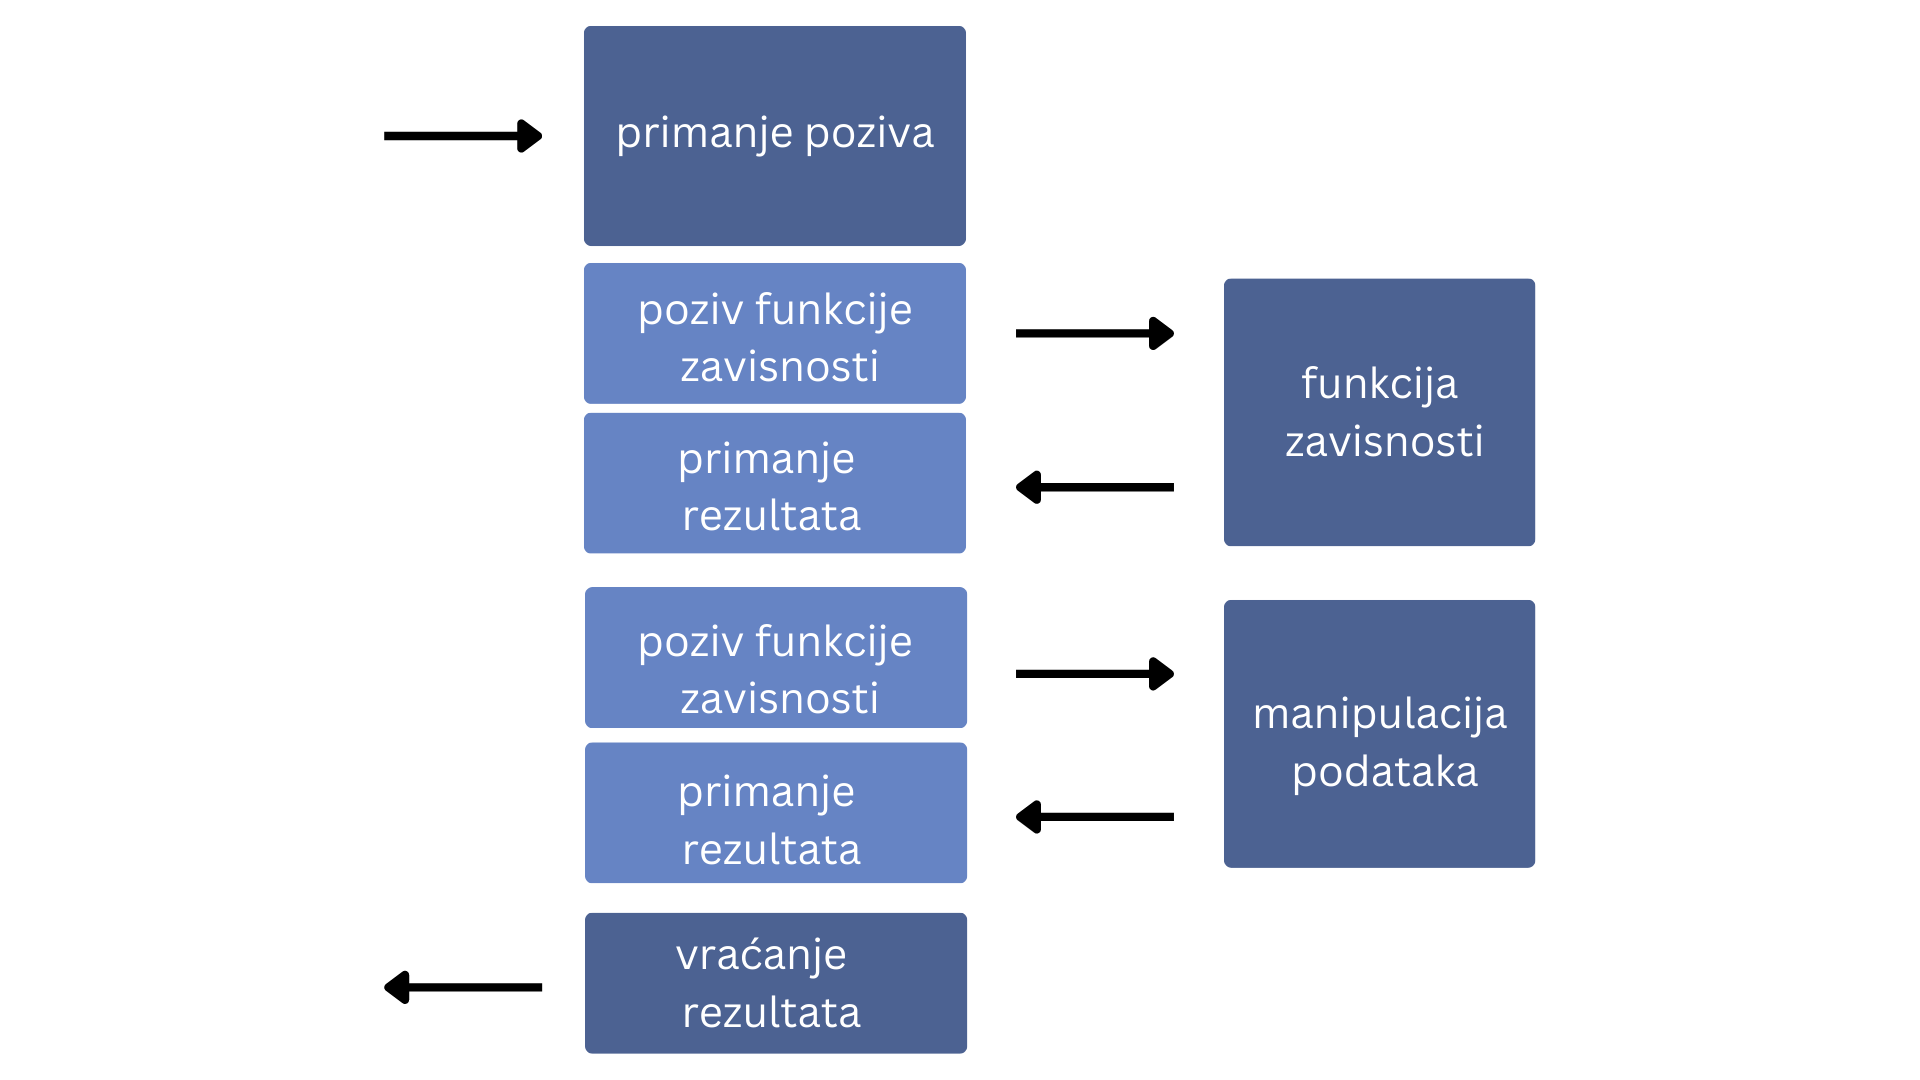
\includegraphics[width=0.6\textwidth]{dep2.png}
  \caption{Nakon izmeštanja u čistu funkciju}
\end{figure}

\par  U nekim slučajevima, nije lako odrediti šta se može izdvojiti u zasebnu funkciju. Tada postoji druga opcija za kreiranje kontrolisanog okruženja: napraviti zamenu za funkciju zavisnosti, i time izolovati kod. 

\subsubsection{Izolovanje koda} 
\par Ubrizgavanjem zavisnosti i kreiranjem osnovnih zamena koje se nazivaju test dublerima (eng. \emph{test doubles}) moguće je eliminisati spoljašnje promenljive, i time kontrolisati situaciju u kojoj kod koji se testira mora da se nađe. Tako se omogućava očekivanje nekog konkretnog rezultata. 
\par Zavisnost je bilo koji kod na koji se originalni kod oslanja. Korišćenjem DI (skraćenica za Dependency Injection) u testovima se kreiraju zamene zavisnosti koje se ponašaju na predvidljiv način, pa testovi mogu da se fokusiraju na logiku unutar koda koji se testira. U jediničnim testovima, najčešće se ubrizgava zavisnost tako što se prosledi kao parametar. Taj parametar može biti funkcija ili modul. Ubrizgavanje zavisnosti kroz API\footnote{skraćenica za aplikacioni veb interfejs (eng. \textit{Web Appilicatoin
Programming Interface} )} je moguće kod jediničnih testova. Omogućava čistoću koda i jednostavne i kontrolisane testove. Sa druge strane, integracioni testovi zahtevaju drugačije metode ubrizgavanja zavisnosti, o čemu će biti više reči u odeljku \ref{sec:integration}.

%TODO
\par TODO ovde ide jos....
% ------------------------------------------------------------------------------

\chapter{Portal MSNR}
\label{chp:msnr}

%TODO 
\par Ovde ide opis aplikacije koja se testira.... \cite{msnr-portal} \cite{rad}

\par Testiranje različitih slojeva aplikacije MSNR portal će u nastavku rada biti sprovedeno u narednim koracima. Za početak će se testirati individualne funkcije i upravljači koji barataju zahtevima i odgovorima u okviru koda za serverski deo aplikacije napisanog u Elixir programskom jeziku pomoću razvojnog okvira Phoenix. Nakon toga, potrebno je testirati integraciju aplikacionog interfejsa sa bazom podataka - integracioni testovi koji simuliraju zahteve API-ju i verifikuju odgovore od baze. TODO jos ovde o tome .... 

\chapter{Testiranje serverskog dela aplikacije}
\label{chp:elixir}
Serverski deo aplikacije MSNR portal napisan je na programskom jeziku Elixir. Elixir je vrlo specifičan jezik, sa konceptima koji mogu biti komplikovani za testiranje. Konkurentost i imutabilnost kao osobine su prisutne i u drugim jezicima, ali na primer rezilijentnost ili OTP (eng. {Open Telecom Platform}) razvojni okvir su vrlo jedinstveni za Elixir (i Erlang). Elixir se prevodi na isti bajtkod kao i Erlang, i pokreće se na Erlang virtuelnoj mašini, poznatoj pod nazivom BEAM.. . jos o elixiru ... Referenca na zvaničnu stranicu \cite{elix} TODO %TODO REF. 
U većini slučajeva, kod napisan u Elixir-u zavisi od nekoliko Erlang biblioteka. Međutim, kada je testiranje koda u pitanju, alati i biblioteke koji se koriste su jedinstveni za svaki od ova dva jezika. Ovde će se govoriti o testiranju isključivo Elixir koda. 

Zajedno sa ovim jezikom dolazi njegov razvojni okvir za testiranje, ExUnit \cite{exunit}. U ovom poglavlju biće predstavljeni različiti koncepti testiranja u programskom jeziku Elixir, kroz pisanje testova za serverski deo aplikacije MSNR portal. Na primeru ove aplikacije, objašnjeni su načini pisanja testova za funkcionalni kod. U narednim sekcijama, prikazano je testiranje važnih osobina Elixir programskog jezika, kao što su tipovi podataka, OTP razvojni okvir, Ecto \cite{ecto}, Phoenix razvojno okruženje\cite{phoenix}.

\section{Testiranje jedinica koda}

Jedinica je mala logička celina koda: može biti funkcija, klasa, metod neke klase, modul i slično. Jedinični test proverava samo da li se data jedinica ponaša prema svojoj specifikaciji. Ovi testovi se mogu pisati u potpunoj izolaciji, i ne zavise ni od jedne druge komponente, servisa, ni korisničkog interfejsa. Dakle, izdvajaju se najmanji testabilni delovi aplikacije i proverava se da li rade ono za šta su namenjeni. Ovi testovi su najjednostavniji za pisanje jer se bave malim delom aplikacije, te je kompleksnost koda koji se testira jako mala. Kao što je navedeno u \ref{sec:piramid}, preporučuje se da ih bude što više kako bi se pokrili svi slučajevi upotrebe.

\textit{ExUnit} je Elixir-ov ugrađeni razvojni okvir koji ima sve što je neophodno za iscrpno testiranje koda i biće osnova za sve testove kroz ovo poglavlje. S obzirom na to da je Elixir funkcionalni jezik, može se diskutovati o tome šta se smatra "jedinicom". Uobičajeno je da se jedinični testovi fokusiraju na pojedinačnu funkciju i njenu logiku, kako bi se opseg testa održavao što užim, radi bržeg pronalaženja grešaka. Međutim, nekada ima smisla da se u opseg testa uključi više modula ili procesa, i time se proširi definicija jedinice koda. Znati kada treba proširiti taj opseg može mnogo uticati na smanjivanje kompleksnosti i održavanje samih testova. 

Pre samog pisanja testova, neophodno je naglasiti ciljeve o kojima je potrebno razmišljati pri dizajniranju testova: 
\begin{enumerate}
\item Dokazati da kod radi ono za šta je namenjen
\item Sprečiti greške (breaking changes - regressions)
\item Utvrditi lokaciju dela koda koji pada
\item Napisati najmanju moguću količinu koda za testiranje
\end{enumerate}

\par Odluku o količini koda koja će činiti jednu jedinicu treba da odrede poslednje dve stavke u navedenoj listi. Uloga testova je da zatvore kod koji se testira u crnu kutiju. Ta kutija definiše mesta gde testni kod komunicira sa kodom aplikacije. Kao što je već navedeno, uži opseg olakšava brzo pronalaženje grešaka u kodu, ali mana ovog pristupa je to što se obično napiše jako velika količina koda, što vremenom postane teško za praćenje. Interakcija testova sa kodom aplikacije će nekada zavisiti od nekog drugog dela koda. Na slici \ref{fig:box1} je prikazan dijagram crne kutije oko koda koji se testira. Pošto taj kod zavisi od nekog drugog dela koda, testovi će morati nekako da naglase izolovanje koda. Izolacija koda često može biti vremenski skupa, i može znatno povećati kompleksnost testova. Crna kutija, tj. opseg testova  se može proširiti tako da uključuje i tu zavisnost, što se može videti na slici \ref{fig:box2}.  Ako je kod od koga zavisi kod koji se testira čisto funkcionalan i dobro testiran sam za sebe - u opseg se može dodati i sama ta zavisnost. Ovime se smanjuje količina posla potrebna za izolovanje koda, a zadržava se mogućnost lakog lociranja lošeg koda. Testovi će i dalje biti fokusirani na mali deo koda, ali zbog toga što je kod čisto funkcionalan može se kontrolisati okruženje pod kojim se testira, i samim tim sprečavaju se nekonzistentni rezultati. Ovakvi testovi su jednostavniji za pisanje, održavanje i razumevanje. Kod od koga zavisi kod pod testom je testiran individualno, i to omogućava da se napiše mnogo manje testova, a i dalje pronađe gde je problem ako test padne. Potrebno je pronaći balans i proceniti kada je potrebno uključiti te čisto funkcionalne zavisnosti u opseg testova. 
\par TODO DA LI JE OVO PONAVLJANJE?
%TODO

\begin{figure}[!ht]
  \centering
  \label{fig:box1}
  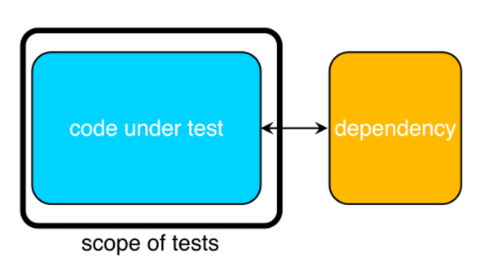
\includegraphics[width=0.4\textwidth]{box1.png}
  \caption{Crna kutija (opseg) oko koda koji se testira}
\end{figure}

\begin{figure}[!ht]
  \centering
  \label{fig:box2}
  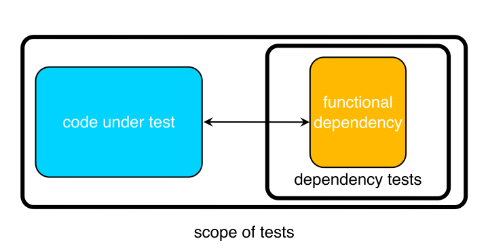
\includegraphics[width=0.4\textwidth]{box2.png}
  \caption{Crna kutija koja uključuje i zavisnosti}
\end{figure}

\par Pisanje testova u programskom jeziku Elixir je moguće bez potrebe za drugim bibliotekama, jer razvojni okvir ExUnit je razvijan zajedno sa samim jezikom od početka. U ovom delu, biće prikazani neki jednostavni jedinični testovi, koji će prikazati neke osnovne koncepte koje nudi ExUnit. 

\subsubsection{Anatomija i organizacija testova}
Svaki jedinični test podeljen je na ne više od četiri faze, ne nužno ovim redosledom:
\begin{enumerate}
\item Priprema (eng. \emph{Setup}) - sređivanje podataka koji će se prosleđivati pred samu proveru, često nije neophodna u testiranju čisto funkcionalnih programa.
\item Delovanje (eng.\emph{Exercise}) - pozivanje koda koji se testira, ključni deo svakog testa.
\item Verifikacija (eng. \emph{Verify}) - često deo prethodne faze, u ovom delu testovi proveravaju ponašanje koda. 
\item Rušenje (eng. \emph{Teardown}) - vraćanje podataka na prvobitno stanje, npr. ako se u prvoj fazi koriste neka deljena stanja, kao što je baza podataka. Često automatski. 
\end{enumerate}

\par Svita testova (eng. \emph{Test suite}) je kolekcija testova slučajeva upotrebe, koji imaju isti posao, ali različite scenarije. Ona može služiti kao dokumentacija, sa opisima o očekivanom ponašanju koda, tako da treba voditi računa da bude dobro organizovana. ExUnit dolazi sa veoma korisnim funkcijima i makroima koji omogućavaju tu organizaciju u jednu čitljivu i održivu  datoteku. Alat \emph{describe } omogućava davanje opisa grupe testova, kao i dodeljivanja zajedničke pripreme podataka za celu grupu. Preporuka je za početak grupisati testove po funkciji, kao što je prikazano u primeru koda \ref{lst:desc}, ali odluka o načinu grupisanja je na pojedincu. Svrha je čitljivost i lakše razumevanje. 

\begin{lstlisting}[language=elixir, caption={Opisivanje testova unutar jedne grupe},captionpos=b, label={lst:desc}]
defmodule MyApp.ModuleTest do 
   use ExUnit.Case 
   
   describe ''thing_to_do/1'' do
   	test ''it returns :ok, calls the function if the key is correct''
   	test ''it does not call the function if the key is wrong''
   end
end
\end{lstlisting}

\par Testovi u Elixir projektima se uglavnom čuvaju u direktorijumu projekta \textit{'/test'}, i organizuju se u module i test slučajeve. U prethodnom primeru koda, modul pod nazivom ModuleTest se sastoji od dva test slučaja. 

\subsection{Pisanje ExUnit testova}
\par Za svaku funkciju ili upravljač potrebno je napisati test slučajeve. Jedan test slučaj se sastoji iz funkcije testa koja poziva funkciju ili upravljač i proverava očekivani rezultat.  



\par ovde jos ... , primeri , ... 


\section{Integraciono testiranje}
\label{sec:integration}
\par Nakon dobro istestiranih pojedinačnih funkcija i modula, potrebno je proveriti da li sistem funkcioniše ispravno kao celina. U ovom poglavlju biće prikazani testovi koji proveravaju da li različiti delovi sistema koji komuniciraju međusobno, kao i sa neki eksternim sistemima, rade to na ispravan način. 
\par Testovi koji pokrivaju integraciju različitih komponenti iste aplikacije ili integraciju aplikacije sa nekim spoljašnjim sistemima nazivaju se \emph{ integracioni testovi}.  Oni su fundamentalni deo testiranja nekog sistema. 
\par Ako se komponente nalaze u okviru istog sistema, gde postoji kontrola i neko očekivano ponašanje - integracioni testovi su prilično jednostavni. Međutim, kada su u pitanju spoljašnje komponente i testiranje interakcije sistema sa njima, pisanje integracionih testova postaje malo komplikovanije. Mnoge aplikacije koriste baze podataka, druge servise ili API-je, sa kojima se testovi moraju uskladiti. U testovima se mogu koristiti prave zavisnosti, ili se umesto njih ubaciti dubleri.
\par Na primer, ako se koristi baza podataka kao spoljašnja komponenta, može se pokrenuti prava baza i pozvati pri izvršavanju testa. Ovakav test obezbeđuje visoko poverenje u ispravnost koda, jer radi kao što bi radio u produkciji. Mana ovog pristupa je brzina - ovi testovi su dosta sporiji od onih koji ne pozivaju zapravo spoljašnje komponente. Baza podataka je komponenta koja se može kontrolisati. U tom slučaju, savetuje se korišćenje pravih komponenti u testovima, kako bi testovi bili što bliži kodu koji će raditi u produkciji. Baza se može pokretati i zaustavljati kada god je neophodno, podaci se mogu menjati po želji, pa se u tim slučajevima žrtvuje brzina izvršavanja testova zarad sigurnosti u ispravnost koda.
\par Sa druge strane, postoje spoljašnje komponente koje su pod tuđim vlasništvom, kao što su neki nezavisni API-ji (eng. \emph{third party API}). Komponenta koja se ponaša kao prava spoljašnja komponenta se naziva dubler te komponente. Pozivaocu ona izgleda isto kao i prava. Nekada ona ne radi ništa, a nekada služi kao uvid u način na koji se ona poziva. Ako se koristi neki spoljašnji API nad kojim ne postoji kontrola, može se desiti da je on ugašen i pri pokretanju automatskih testova, oni ne prolaze. Iz tog razloga, preporuka je da se u testovima izbegne direktno kontaktiranje tog API-ja. Najjednostavniji način je ubrizgavanje zavisnosti, prethodno spomenuto u delu \ref{sec:piramid}. Interfejsi se često enkapsuliraju u module, pa ovde ima smisla ubrizgati modul kao zavisnost. U produkciji bi se koristio pravi modul API-ja, a tokom testiranja pozivao bi se lažni modul.

\subsection{Test dubleri}
Dubleri se mogu podeliti na 3 vrste:  (eng. stubs), (eng. mocks) i  (eng. fakes). 
\par Stub ....v

\subsection{Neki podnaslov}
U aplikaciji MSNR portal - TODO konkretni primeri ... 

\chapter{Testiranje klijentskog dela aplikacije}
\label{chp:elm}

\chapter{Integracija klijentske i serverske strane}
\label{chp:elmelixir}

\chapter{Testiranje celokupnog sistema - End to End}
\label{chp:e2e}

% ------------------------------------------------------------------------------
\chapter{Zaključak}
% ------------------------------------------------------------------------------

% ------------------------------------------------------------------------------
% Literatura
% ------------------------------------------------------------------------------
\literatura

% ==============================================================================
% Završni deo teze i prilozi
\backmatter
% ==============================================================================

% ------------------------------------------------------------------------------
% Biografija kandidata
%\begin{biografija}

%\end{biografija}
% ------------------------------------------------------------------------------

\end{document}
